
%%%%%%%%%%%%%%%%%%%%%%%%%%%%%%%%%%%%%%%%%%%%%%
\chapter{Классификация алгоритмов}

Способы классификации алгоритмов были взяты из \cite{DBLP:journals/corr/abs-2011-00583}. Алгоритмы, рассмотренные ниже, не были полностью классифицированы в статье.
Классификация алгоритмов MARL зависит от типа проблемы, а не от подхода к решению, как в области обучения с подкреплением. 

\section{Классификация согласно теории обучения с подкреплением}

Классификация по типу действий в среде:
\begin{itemize}[label=---]
	\item дискретное действие - прим: Atari дискретными кнопками; 
	\item непрерывное действие - прим: Doom с аналоговым вводом мышки.
\end{itemize}

По необходимости непосредственного взаимодействия агента со средой:
\begin{itemize}[label=---]
	\item необходимо непосредственное взаимодействие агента - On Policy;
	\item может учиться по записям игр - Off Policy.
\end{itemize}

% Please add the following required packages to your document preamble:
% \usepackage{booktabs}

Таблица \ref{classification} показывает классификацию алгоритмов MARL по необходимости непосредственного взаимодействия агента со средой, по типам обучения.

\begin{table}[H]
	\centering
	\caption{Классификация алгоритмов MARL по необходимости непосредственного взаимодействия агента со средой, по типам обучения}
	\label{classification}
	\begin{tabular}{@{}|l|l|l|l|l|@{}}
	\toprule
	Алгоритм & Центр. Обучение & On/Off Policy & Q--обучение     & Учит стратегию \\ \midrule
	IQL      & x          	   & Off           & \checkmark     & x             \\
	VDN      & \checkmark      & Off           & \checkmark     & x              \\
	QMIX     & \checkmark      & Off           & \checkmark     & x              \\
	MAVEN    & \checkmark      & Off           & \checkmark     & x              \\
	MADDPG   & \checkmark      & Off           & \checkmark     & \checkmark     \\
	IPPO     & x  		       & On            & \checkmark     & \checkmark     \\
	MAPPO    & \checkmark      & On            & \checkmark     & \checkmark     \\
	\bottomrule
	\end{tabular}
\end{table}

Алгоритмы, которые не обучают стратегию, не могут быть применены к играм с континуальным пространством действий. 


\section{Классификация по типу игры}

Типы игр были описаны ранее. Приведем их здесь для ссылки:
\begin{itemize}[label=---]
	\item кооперативные игры (Cooperative Games);
	\item соревновательные игры (Competitive Games);
	\item смешанные игры (Mixed Games).
\end{itemize}

Рассматриваемые алгоритмы достаточно общие и могут быть применены ко всем типам игр.
Тем не менее, существуют другие, не рассматриваемые алгоритмы, которые специализируются на определенных типах игр.

%\section{Классификация по уровню локальных знаний}
%
%Алгоритмы можно классифицировать по уровню локальных знаний - количеству информации, известному агенту во время обучения.
%
%Выделим следующие уровни информации:
%
%\begin{enumerate}[label={\arabic*)}][label=\arabic*)]
%	\item агент наблюдает награду за совершенное действие;
%	\item агент может наблюдать награду за все действия;
%	\item агент может наблюдать действия других агентов;
%	\item агент может наблюдать V-функцию других агентов;
%	\item агент знает стратегию других агентов;
%	\item агент знает функцию наград других агентов;
%	\item агент знает, где находится эквилибриум.
%\end{enumerate}
%
\section{Классификация по парадигме обучения}

\begin{figure}[H]
	\begin{center}
	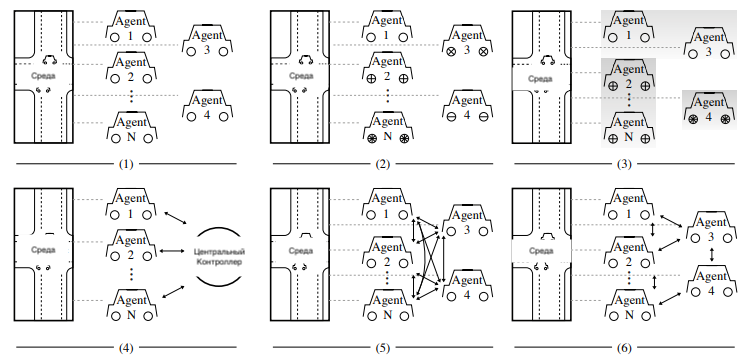
\includegraphics[pages=-, width=140mm]{./inc/img/paradigm.png}
	\caption{Классификация по парадигме обучения}
	\label{fig:paradigms}
\end{center}
\end{figure}


Различают следующие парадигмы обучения \cite{DBLP:journals/corr/abs-2011-00583}:
\begin{enumerate}[label=\arabic*)]
	\item независимые агенты с общей стратегией;
	\item независимые агенты с независимой стратегией;
	\item независимые агенты с общей стратегией внутри команды;
	\item один контроллер всех агентов;
	\item во время обучения агенты централизованны, а во время тестирования децентрализованы;
	\item во время обучения агенты децентрализованы, но могут обмениваться сообщениями в сети, во время тестирования децентрализованы.
\end{enumerate}


% Please add the following required packages to your document preamble:
% \usepackage{booktabs}

Таблица \ref{tab:paradigms} содержит классификацию алгоритмов по парадигме обучения.

\begin{table}[H]
	\centering
	\caption{Классификация по парадигме обучения}
	\label{tab:paradigms}
	\begin{tabular}{@{}|l|l|@{}}
	\toprule
	Алгоритм & Парадигма \\ \midrule
	IQL      & 2         \\
	VDN      & 2         \\
	QMIX     & 2         \\
	MAVEN    & 2         \\
	MADDPG   & 5         \\ 
	IPPO     & 1 или 2   \\
	MAPPO    & 5         \\
	\bottomrule
	\end{tabular}
\end{table}

\subsection*{Вывод}

Были предложены методы классификации алгоритмов, алгоритмы классифицированы согласно предложенным методам.

% обобщение и оценку результатов исследований, включающих оценку полноты решения поставленной 
% задачи и предложения по дальнейшим направлениям работ, оценку достоверности полученных
% результатов и технико-экономической эффективности их внедрения и их сравнение с аналогичными
% результатами отечественных и зарубежных работ, обоснование необходимости проведения дополнительных 
% исследований, отрицательные результаты, приводящие к необходимости прекращения дальнейших исследований.

Существует множество алгоритмов обучения агентов в среде с несколькими агентами.
Следует помнить что оптимальная стратегии для одного агента может быть не оптимальной для нескольких агентов в совокупности.
Не все рассматриваемые алгоритмы гарантируют сходимость к оптимальной стратегии, то есть предоставляют теоретическую гараантию решения проблемы.

Существуют другие дисциплины обучения с подкреплением, например обратное обучение, когда агенту не дают награды. В дальнейших работах было бы интересно рассмотреть эти алгоритмы.